\chapter{Work Done till Stage Zero} \label{ch3}
For future work in the dual degree project, COMSOL Multiphysics 5.3 software will be used. Before moving forward different solving techniques and schemes have to be verified against benchmark results which will be used for further analysis. The aim is to reproduce the results that already exist in the literature which is used widely for verification. Two studies will be performed for this verification. The First study will be based solely on natural convection while the second study will include both natural convection with radiation.
\section{Verification for a Natural Convection Problem}
For verification of natural convection, the problem is given by de Vahl Davis\citep{de1983natural} has been used which includes natural convection inside a square cavity in which left and right walls are maintained at a different temperature. Many researchers working on natural convection have used its solution as a bench mark. The problem statement followed by the comparison of result has been given in this chapter.
\subsection{Problem Statement}\label{cov_prob_st}
The fluid fills a square cavity with impermeable walls so the fluid flows freely within it but does not exit from it. The right and left edges of the cavity are, respectively, the high and low temperature sources. The upper and lower boundaries are insulated as shown in the figure\ref{convpic}. The temperature differential produces the density variation that drives the buoyant flow. The cavity is filled with Boussinesq fluid of Prandtl number 0.71. It has a side length of $L$ and no-slip boundary condition has been used at all the four boundaries.\\

\begin{figure}[H]
\begin{center}
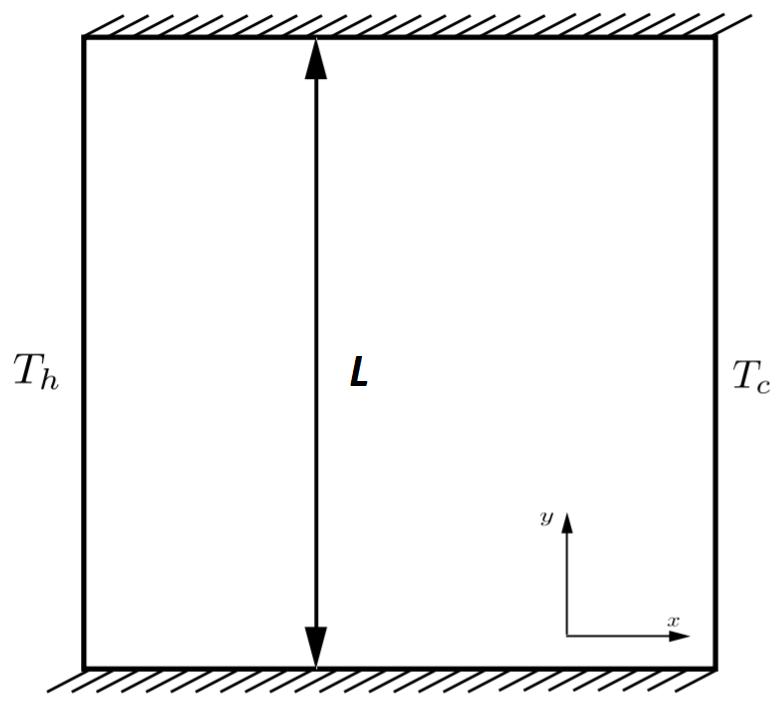
\includegraphics[width = 0.4\textwidth]{convpic.PNG}
\caption{Square cavity}
\label{convpic}
\end{center}
\end{figure}




After non-dimensionalizing Navier-Stokes equation with characteristic length $L$ non-dimensional numbers are obtained. Thsese numbers are called Rayleigh ($Ra$) and Prandtl number (Pr) respectively which can be expressed as
\begin{equation}
Ra = \frac{g\beta(T_h-T_c)L^3 Pr}{\nu^3} \qquad and \qquad Pr = \frac{\nu}{\alpha}
\end{equation}

Described model is solved with the Laminar Flow and the Heat Transfer in Fluids interfaces available in COMSOL Multiphysics 5.3. For the Navier-Stokes equations, impermeable, no slip boundary conditions is applied. The no slip condition implies that velocity at the wall is zero. Body force in x-direction $F_x$ is zero and y-direction  is set to $F_y = Ra Pr T'$ for momentum equation. 
\subsection{Meshing}
To create mesh in-built options for element size has been used. Predefined option of extra fine element size has been selected in the area while on the hot and cold walls extremely fine element size has been taken.
\subsection{Results}
Study has been performed for different values of Rayleigh number given in table \ref{nu}. A comparison of average Nusselt number obtained by described simulation has been shown against values given by Vahl Davis\citep{de1983natural} with percentage deviation.
% Please add the following required packages to your document preamble:
% \usepackage{multirow}
\begin{table}[H]
\centering
\caption{Comparison of computed average Nusselt number with benchmark result}
\label{nu}
\begin{tabular}{|c|c|c|c|}
\hline
\multirow{2}{*}{\textbf{Ra}} & \multicolumn{2}{c|}{\textbf{Average Nusselt Number}}       & \multirow{2}{*}{\textbf{\% Deviation}} \\ \cline{2-3}
                             & \textbf{Computed} & \textbf{Vahl Davis} &                                        \\ \hline
10$^3$                     & 1.116             & 1.117               & 0.090                                  \\ \hline
10$^4$                     & 2.242             & 2.244               & 0.089                                  \\ \hline
10$^5$                     & 4.523             & 4.521               & 0.044                                  \\ \hline
10$^6$                     & 8.928             & 8.831               & 1.086                                  \\ \hline
\end{tabular}
\end{table}

Comparisons of streamline function, horizontal direction velocity, vertical direction velocity and temperature contours for Rayleigh number $10^6$ has been shown.

\begin{figure}[H]
  \centering
  \begin{minipage}[b]{0.45\textwidth}
    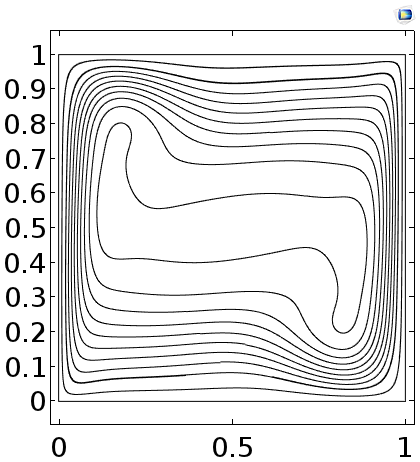
\includegraphics[width=\textwidth]{streamf_Ra_1E6.png}
    \caption{Streamline function from simulation}
  \end{minipage}
  \hfill
  \begin{minipage}[b]{0.5\textwidth}
    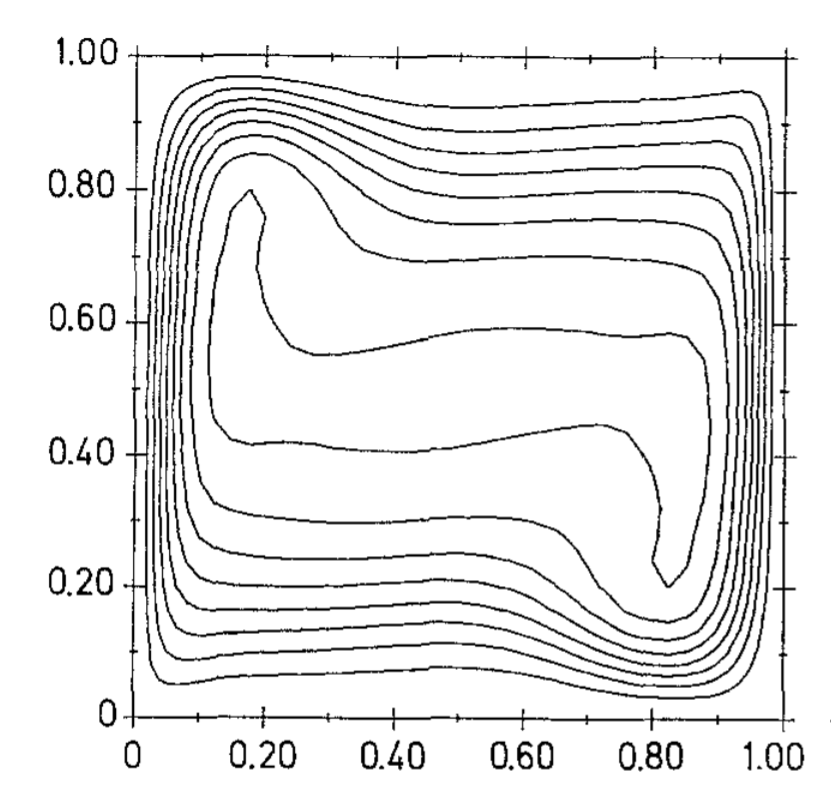
\includegraphics[width=\textwidth]{streamlineRa1e6benchmark.PNG}
    \caption{Streamline function from benchmark solution}
  \end{minipage}
\end{figure}

\begin{figure}[H]
  \centering
  \begin{minipage}[b]{0.5\textwidth}
    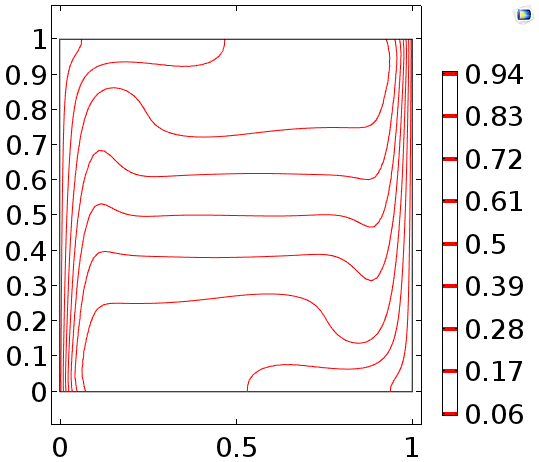
\includegraphics[width=\textwidth]{T_Ra_1E6.png}
    \caption{Temperature contours from simulation}
  \end{minipage}
  \hfill
  \begin{minipage}[b]{0.4\textwidth}
    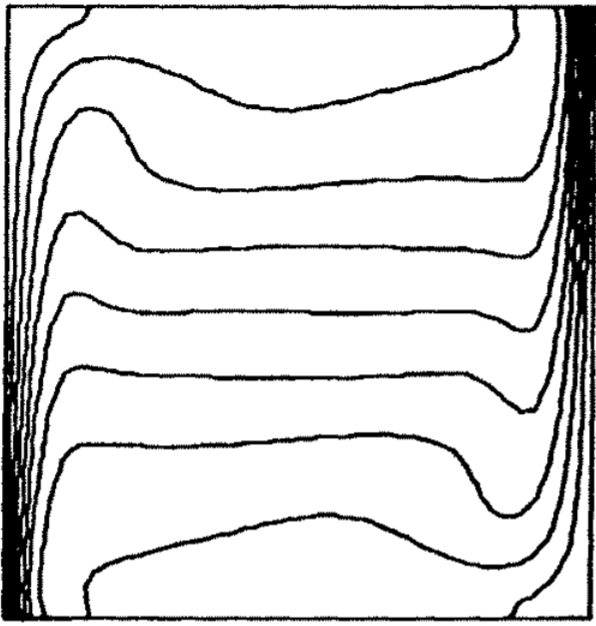
\includegraphics[width=\textwidth]{Tcontours.PNG}
    \caption{Temperature contours from benchmark solution}
  \end{minipage}
\end{figure}

\begin{figure}[H]
  \centering
  \begin{minipage}[b]{0.5\textwidth}
    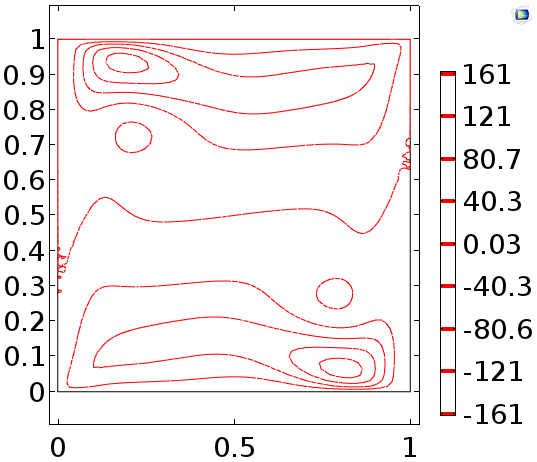
\includegraphics[width=\textwidth]{u_Ra_1E6.png}
    \caption{Horizontal velocity contours from simulation}
  \end{minipage}
  \hfill
  \begin{minipage}[b]{0.4\textwidth}
    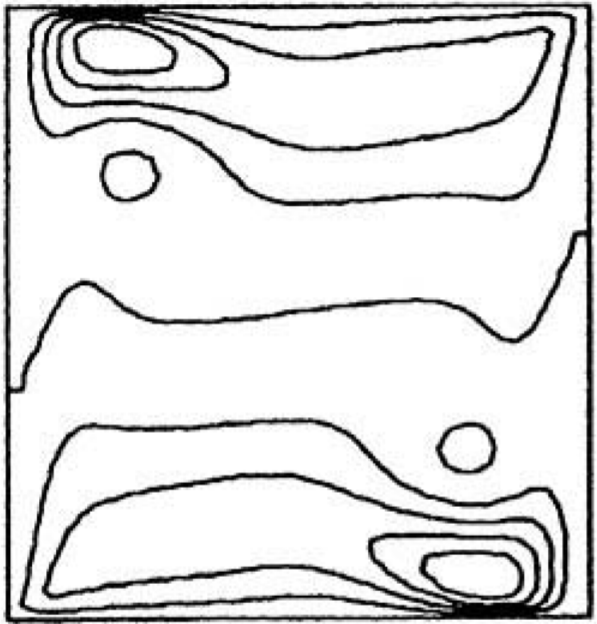
\includegraphics[width=\textwidth]{ucontour.PNG}
    \caption{Horizontal velocity contours from benchmark solution}
  \end{minipage}
\end{figure}

\begin{figure}[H]
  \centering
  \begin{minipage}[b]{0.5\textwidth}
    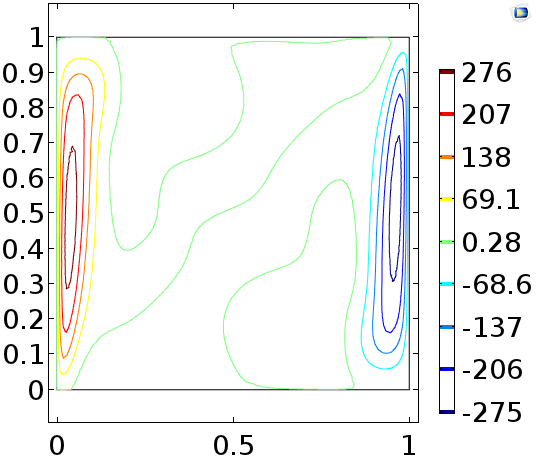
\includegraphics[width=\textwidth]{v_Ra_1E6.png}
    \caption{Vertical velocity contours from simulation}
  \end{minipage}
  \hfill
  \begin{minipage}[b]{0.4\textwidth}
    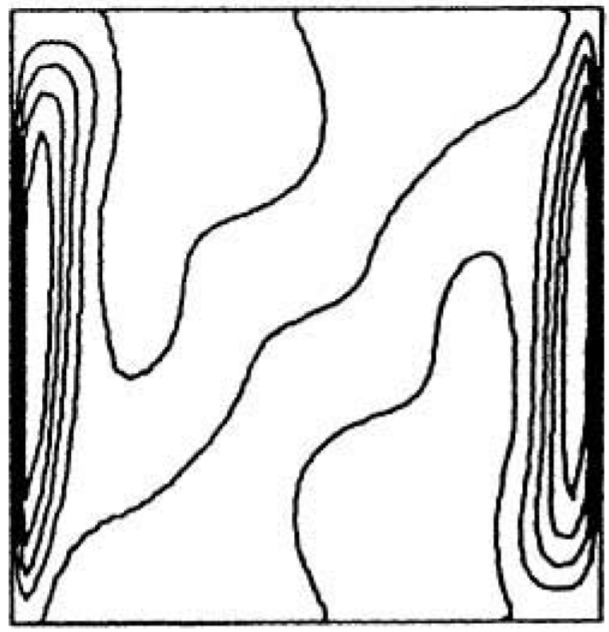
\includegraphics[width=\textwidth]{vcontour.PNG}
    \caption{Vertical velocity contours from benchmark solution}
  \end{minipage}
\end{figure}



Since computed results are in good agreement with the benchmark solution it is concluded that numerical scheme used for simulation of natural convection problem is verified.
\chapter{Work Done after Stage Zero}
\section{Natural Convection in a Trapezoidal Cavity}
This section describes study performed in COMSOL Multiphysics 5.3for natural convection in a trapezoidal cavity. Result obtained from this study is compared with M. Tech. thesis of Sarath Mohan. 
\subsection{Problem Statement}
Top surface of the trapezoidal cavity is maintained at a constant temperature, bottom surface is subjected to natural convection and radiation to ambient, rest of two surfaces are insulated. No slip condition is valid at all the four boundaries. Geometry is described in the figure \ref{fig:geometry modified}. Heat transfer coefficient of $25\ W/m^2$ with ambient temperature $300\ K$ is defined for natural convection. Emissivity of $0.9$ for bottom wall is defined for radiation to ambient.

\begin{figure}[H]
\begin{center}
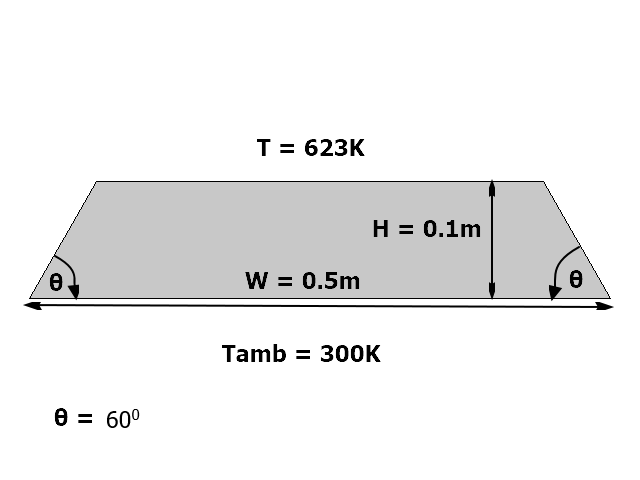
\includegraphics[width = 0.6\textwidth]{geometry_modified.png}
\caption{Trapezoidal cavity geometry}
\label{fig:geometry modified}
\end{center}
\end{figure}
\subsection{Meshing}
Predefined element size in COMSOL has been used for simulating this model. fine element size is used for inner domain and side walls while extremely fine element size is used for top and bottom walls.

\subsection{Result and Verification}
Isothermal contour obtained from simulation has been shown in figure \ref{fig:isotherms trapz cavity} which shows temperature variation in the cavity. Total heat transfer from the hot wall and average Nusselt number at the hot wall is calculated and compared against M. Tech. thesis of Sarath Mohan in table \ref{tab:conv trapz cavity}.



% Please add the following required packages to your document preamble:
% \usepackage[table,xcdraw]{xcolor}
% If you use beamer only pass "xcolor=table" option, i.e. \documentclass[xcolor=table]{beamer}
\begin{table}[H]
\centering
\caption{Result verification for trapezoidal cavity}
\label{tab:conv trapz cavity}
\begin{tabular}{|c|c|c|}
\hline
\textbf{Parameters} & \textbf{COMSOL} & \textbf{M. Tech thesis} \\ \hline
Heat (W)                                    & 50.77           & 50.06                   \\ \hline
Nusselt Number                              & 1.02            & 1.12                    \\ \hline
\end{tabular}
\end{table}


\begin{figure}[H]
\begin{center}
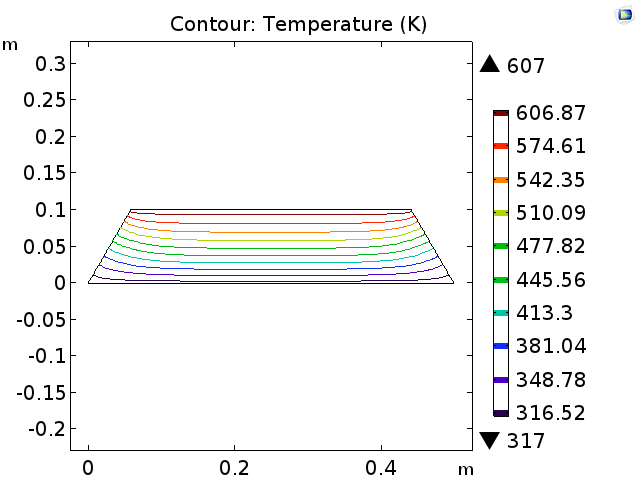
\includegraphics[width = \textwidth]{Isothermal_contour_convection.png}
\caption{Isothermal contour in trapezoidal cavity}
\label{fig:isotherms trapz cavity}
\end{center}
\end{figure}



\section{Verification for a combined radiation convection problem}
In a square cavity, the interaction between radiation and natural convection has been studied by Balaji and Venkateshan \citep{BALAJI1994249}. Even at the low emissivity of walls, radiation has a significant impact on natural convection inside the cavity. Correlations for the radiative Nusselt number and the convective Nusselt number have been provided by them. They were able to show that when radiation increases, convective Nusselt number decreases but overall Nusselt number which is the sum of both the Nusselt numbers can either go up or down depending on the other parameters. So, it should be made sure that mathematical models and numerical schemes which are going to be used for further study accommodate these effects. The problem is modeled in COMSOL and simulated for the result. Simulation work is still in progress. The solution obtained will be verified against the results obtained by Balaji and Venkateshan \citep{BALAJI1994249} which will serve as the benchmark for the verification.
\subsection{Problem statement}
The geometry of the cavity is same as described in subsection\ref{cov_prob_st}. Boundary conditions are similar as well except that at the insulated walls heat conducted is equal to net radiation heat transfer making total heat transfer equal to $0$. In literature most commonly used radiation modeling technique is S2S (surface to surface) where the medium is non-participant in radiation heat transfer. That is scattering, absorption and emission by participating medium is not considered. This method is also based on view factor calculation between surfaces. But it is found that it does not give accurate results and show oscillations in
case of symmetric planes. This issue is also mentioned by Pye\citep{pye2003modelling}. Thus a more accurate radiation model DO (Discreet ordinate) will be used. Simulations will be performed for different values of wall emissivity and compared with benchmark results.

\chapter{Ray Optics}\label{ch5}
LFR system is governed by physics of fluid flow, heat transfer and ray optics. To study LFR model in COMSOL Multiphysics 5.3, physics modules related to concerned physics have to be used together. Study related to fluid flow and heat transfer has been performed in the software and verified against benchmark in chapter \ref{ch3}. This chapter describes study and simulation performed using Ray Optics module in COMSOL Multiphysics 5.3.
\section{Problem Statement}\label{sec:ps rayops}
A fully polarized parallel beam of light is falling on two reflecting surfaces and after reflection it reaches to a receiver where it is absorbed. Geometry can be seen in the figure \ref{fig:geo ray ops} where 'B' and 'C' are reflective surfaces and 'A' is the receiver which absorbs all the rays falling on it. Geometry for this study has been constructed in such a way that middle point of reflective surfaces 'B' and 'C' lie on a parabola and focus of this parabola lies on the middle point of the receiver 'A'. So that parallel beams coming along the axis of this parabola, converges at the middle point of the receiver. 
\begin{figure}[H]
  \centering
  \begin{minipage}[b]{0.4\textwidth}
    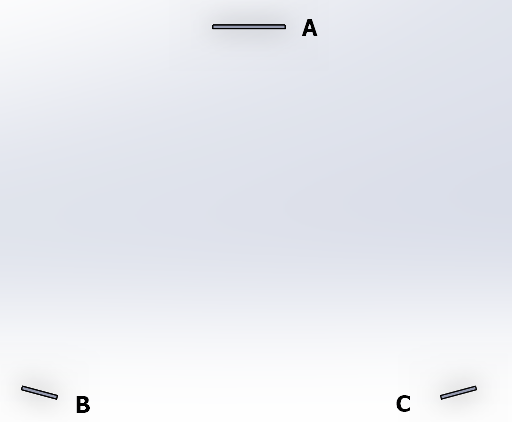
\includegraphics[width=\textwidth]{cad_model_ray_optics_front_view.PNG}
    \caption{Front view}
  \end{minipage}
  \hfill
  \begin{minipage}[b]{0.4\textwidth}
    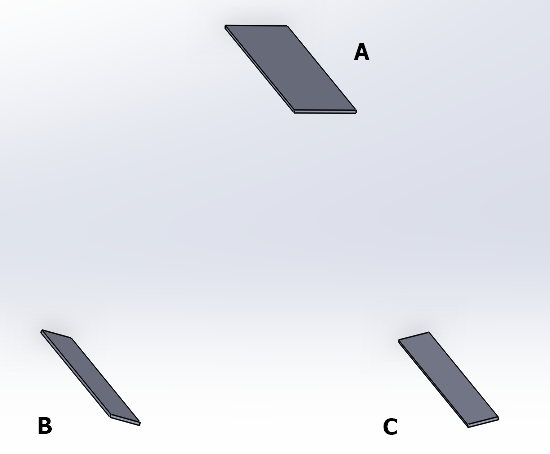
\includegraphics[width=\textwidth]{cad_model_ray_optics_side_view.PNG}
    \caption{Isometric view}
  \end{minipage}
  \label{fig:geo ray ops}
  \caption{Geometry used for ray optics simulation}
\end{figure}
Source power of $10\ W$ has been used to generate parallel beam of light which is monochromatic in nature. Ray trajectories and heat flux on the receiver have been obtained as output of the simulation. Two variants of this simulation have been done. In the first case reflective surfaces are assumed to be ideal which reflects everything falling on them and does not absorb anything. But in reality certain fraction of the incoming radiation is absorbed by the reflector itself. Even in the case of newly installed reflectors a significant fraction is absorbed. Over the years after installation due to wear and tear absorbed fraction increases. To account for this absorption, another simulation has been performed in which absorption coefficient of $0.1$ has been defined for both the receivers.
\section{Meshing}
COMSOL Multiphysics 5.3 has different in-built options for element size while meshing. For reflective surfaces 'B' and 'C' fine element size is used. Since absorbed heat flux due to incident rays is being calculated on the receiver 'A', to increase accuracy, extremely fine element size is used for meshing 'A'.
\section{Results}\label{sec:ray ops result}
As described in section \ref{sec:ps rayops} two variants of the simulation have been performed. One is for ideal reflectors and another one for real reflectors and their results are given in this section.

\begin{figure}[H]
\begin{center}
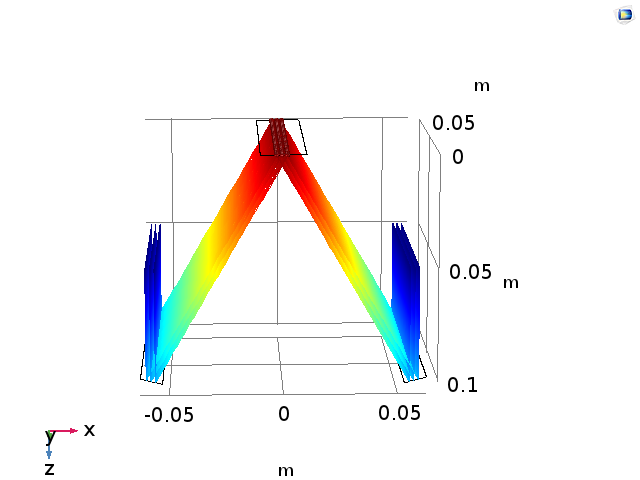
\includegraphics[width = 0.8\textwidth]{ideal_reflector_grid_release_ray_trajectories.png}
\caption{Ray trajectories}
\label{fig:ray ops ray traj}
\end{center}
\end{figure}

Ray trajectories obtained from the simulation can be seen in the figure \ref{fig:ray ops ray traj}. Parallel rays after being reflected by reflective surfaces gets absorbed by the absorber. Heat flux distribution on the absorber in case of ideal and real absorber can be seen in the figures \ref{fig:ray ops heat flux ideal ref} and \ref{fig:ray ops heat flux real ref}.

\begin{figure}[H]
\begin{center}
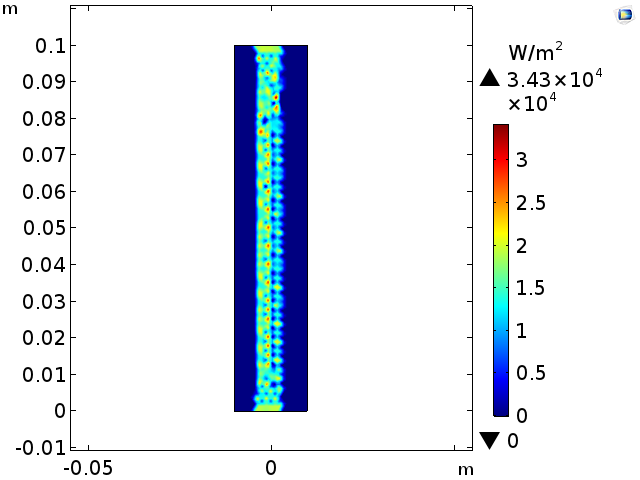
\includegraphics[width = 0.75\textwidth]{Ideal_reflector_grid_release_surface_heat_flux_plot.png}
\caption{Flux distribution for ideal reflector}
\label{fig:ray ops heat flux ideal ref}
\end{center}
\end{figure}

\begin{figure}[H]
\begin{center}
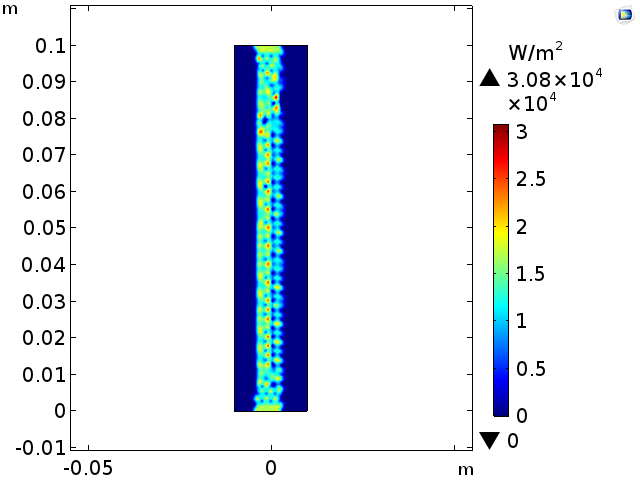
\includegraphics[width = 0.75\textwidth]{Real_reflector_grid_release_surface_heat_flux_plot.png}
\caption{Flux distribution for real reflector}
\label{fig:ray ops heat flux real ref}
\end{center}
\end{figure}
Surface distribution of heat flux is not uniform but small dots can be observed where rays have hit the receiver. It is due the fact that limited number of rays were used for simulation. There are no rays absorbed by the receiver along its two boundaries which can be observed from the two rectangular straps along the length of the receiver depicting heat flux of $0\ W/m^2$. Which concludes that no ray escaped the receiver along its width. Width of the receiver was given by guess so that it can intercept all the rays which it did. Length of the receiver and reflective surfaces were kept the same and incident rays were in the which is perpendicular to both reflectors and the receiver. Which ensures that no ray escaped the receiver along its length. Thus all the rays were intercepted by the receiver. This fact will be helpful in the section \ref{sec:ray ops verf} where result obtained from simulation will be verified against analytical calculation.

Surface average of heat flux obtained on the receiver in case of ideal reflector is $5000\ W/m^2$ while it is $4500\ W/m^2$ in case of real reflectors.

\section{Verification}\label{sec:ray ops verf}
In the section \ref{sec:ray ops result}, we have established the fact that all the incident rays were intercepted by the receiver. In this section average heat flux falling on the receiver will be analytically calculated and result obtained from the simulation will be verified against it.\\
\textbf{Case 1: Ideal reflectors}\\
\begin{align*}
Source\ power:\ P_{source} = 10\ W \\
Area\ of\ the\ receiver:\ A_{rec} = 0.02\times0.1 \ m^2 \\
Absorption\ coefficient:\ \alpha = 0.0 \\
Heat\ flux\ on\ the\ receiver:\ q" = (1-\alpha)\times\frac{P_{source}}{A_{rec}} \\
q" = 5000\ W/m^2
\end{align*}
\textbf{Case 1: Real reflectors}\\
\begin{align*}
Source\ power:\ P_{source} = 10\ W \\
Area\ of\ the\ receiver:\ A_{rec} = 0.02\times0.1 \ m^2 \\
Absorption\ coefficient:\ \alpha = 0.1 \\
Heat\ flux\ on\ the\ receiver:\ q" = (1-\alpha)\times\frac{P_{source}}{A_{rec}} \\
q" = 4500\ W/m^2
\end{align*}


Average heat flux on the receiver obtained from simulation have been compared against analytically calculated values in table \ref{tab:ray ops heat flux}.

% Please add the following required packages to your document preamble:
% \usepackage{multirow}
\begin{table}[H]
\centering
\caption{Comparison of average heat flux}
\label{tab:ray ops heat flux}
\begin{tabular}{|c|c|c|}
\hline
\multirow{2}{*}{\textbf{Reflectors}} & \multicolumn{2}{c|}{\textbf{\begin{tabular}[c]{@{}c@{}}Absorbed heat\\   flux on the receiver ($W/m^2$)\end{tabular}}} \\ \cline{2-3} 
                                     & \textbf{Simulation}                                               & \textbf{Analytical}                                              \\ \hline
Ideal                                & 5000                                                              & 5000                                                             \\ \hline
Real                                 & 4500                                                              & 4500                                                             \\ \hline
\end{tabular}
\end{table}

From table \ref{tab:ray ops heat flux}, it can be concluded that simulation accurately computed the average heat flux on the receiver.





\chapter{Future Work} \label{ch4}
Various studies have been performed related to cavity receivers which include experimental as well as numerical analysis. Researchers have studied this field by varying different parameters and analyzed its effect. Effects of temperature ratio, aspect ratio, the temperature of cavity receivers, the emissivity of different surfaces, Grashof number, the number of tubes etc. has been studied over the years. Effect of evacuated concentric receivers instead of regular receivers and shape of receiver tubes has been analyzed. Cavity simulation with modified geometry has been performed as well which accounts for pipes within the geometry and more accurate results were obtained. Optimization of cavity receiver design has also been studied to minimize overall heat loss recently. Last year, Qiu et.al.\citep{QIU2016129} have developed a model by coupling trapezoidal cavity receivers with linear Fresnel reflectors. They used Finite Volume Method and Monte Carlo ray tracing to study the entire process. Results Monte Carlo ray tracing was converted to Fluent data  by "Coupling Code" and then Finite Volume Method was used solve the heat and flow equations in Fluent. They have coupled two different softwares via "coupling code", which is not always a very easy task and it requires knowledge of coding as well. COMSOL Multiphysics has all the required physics modules to perform this study. Geometrical optics, Fluid flow and Heat transfer equation can be simultaneously solved to perform LFR studies using COMSOL Multiphysics. Since all the required physics modules are internally connected, it completely bypasses the requirement of any coupling code or knowledge of code for that matter, making overall study easier.	 They have studied optical and thermal performances of the system. To solve the model they have used 3-D model which is complex and has more computational cost than a 2-D model. 

With certain approximations, a less complex analysis can be performed with reduced computational cost. Further, effects of various parameters can be studied on this combined model of such as the effect of different wind velocity, the selective coating used for receivers as well as internal walls. Various Correlations can be obtained based on these parameters. By obtaining temperature profile heat losses as a function of length can be obtained which is an important factor in the design of LFR systems\citep{bellos2016experimental}.







%General trends observed in literature review

%State shortcomings of the research/ future work given in papers/challenges


%conclusion - 'these would be the areas on which to concentrate upon'


%%% End: 
